%----------------------------------------------------------------------------------------
%	HEADER IMAGE
%----------------------------------------------------------------------------------------

% \begin{figure}[H]
% \centering
\includegraphics[width=0.3\linewidth]{logo3.png}
% \centering
\includegraphics[width=0.3\linewidth]{logo.png}
% \end{figure}

%----------------------------------------------------------------------------------------
%	SIDEBAR - FIRST PAGE
%----------------------------------------------------------------------------------------

% \begin{minipage}[t]{.30\linewidth} % Mini page taking up 30% of the actual page
\begin{minipage}[t]{.30\linewidth} % Mini page taking up 30% of the actual page

\begin{figure}[H]
\centering
\includegraphics[width=0.9\linewidth]{logo3.png}
\end{figure}

\begin{mdframed}[style=sidebar,frametitle={}] % Sidebar box

%-----------------------------------------------------------

\textbf{{\large What We're Up To}}

\begin{itemize}
    \item Setting up our makerspace and study room
    \item Recruiting new members we are looking at over ten potential members, 6 of whom are especially promising
    \item Our application to be a 501c(3) nonprofit is in the hands of the IRS - expecting approval in February or March
\end{itemize}

\centerline {\rule{.75\linewidth}{.25pt}} % Horizontal line

%-----------------------------------------------------------

\textbf{On Going Projects}

\begin{itemize}
\item Designing luxury furniture for a sponsor
\item Christian running an anime and comic products store
\item Andrew is running an artisan pen company
\item Neil is running a patented knifemaking business
\end{itemize}

%-----------------------------------------------------------

% \centerline {\rule{.75\linewidth}{.25pt}} % Horizontal line

% \textbf{Needs}

% \begin{itemize}
%     \item Funds to cover legal expenses
%     \item Office essentials to stock the study room and makerspace (particularly whiteboards, chairs, and desks) 
%     \item Funds to have a more robust and involved recruitment process for our next recruiting season
%     \item Experienced entrepreneurs to volunteer as guest speakers
% \end{itemize}


\end{mdframed}

\begin{minipage}[t]{0.95\linewidth}
\textbf{Contact Information:}\\
Jack Cooperman \\
\href{mailto:cooperjd@rose-hulman.edu}{cooperjd@rose-hulman.edu} \\
President

Ryan Brown \\
\href{mailto:brownrl@rose-hulman.edu}{brownrl@rose-hulman.edu} \\
Public Relations
\end{minipage}

\centering\includegraphics[width=0.95\textwidth]{housepic2.jpg}
\end{minipage}\hfill % End the sidebar mini page 
% note: do not put a non-comment line between this and the next line, it will put the sidebar on a new
%       page if you do
%----------------------------------------------------------------------------------------
%	MAIN BODY - FIRST PAGE
%----------------------------------------------------------------------------------------
\begin{minipage}[t]{.66\linewidth} % Mini page taking up 66% of the actual page

\customtitle{Who We Are}{6pt}

Delta Rho Sigma is a professional fraternity that focuses on entrepreneurship. We look to provide an environment that helps students integrate an entrepreneurial mindset into their personal talents and high-level engineering and business skills.

%-----------------------------------------------------------

\heading{Startup Weekend}{6pt}

Students from the 2026 ESCALATE class participated in Startup Weekend (Oct. 21-23). Startup Weekend is organized by Techstars, Rose Innovative Student Entrepreneurs (RISE), Delta Rho Sigma, and ESCALATE. The event allowed students to experience what it's like to take an idea and start transforming it into a business. Students were able to speak with mentors and receive feedback to help shape their ideas.

% \begin{center}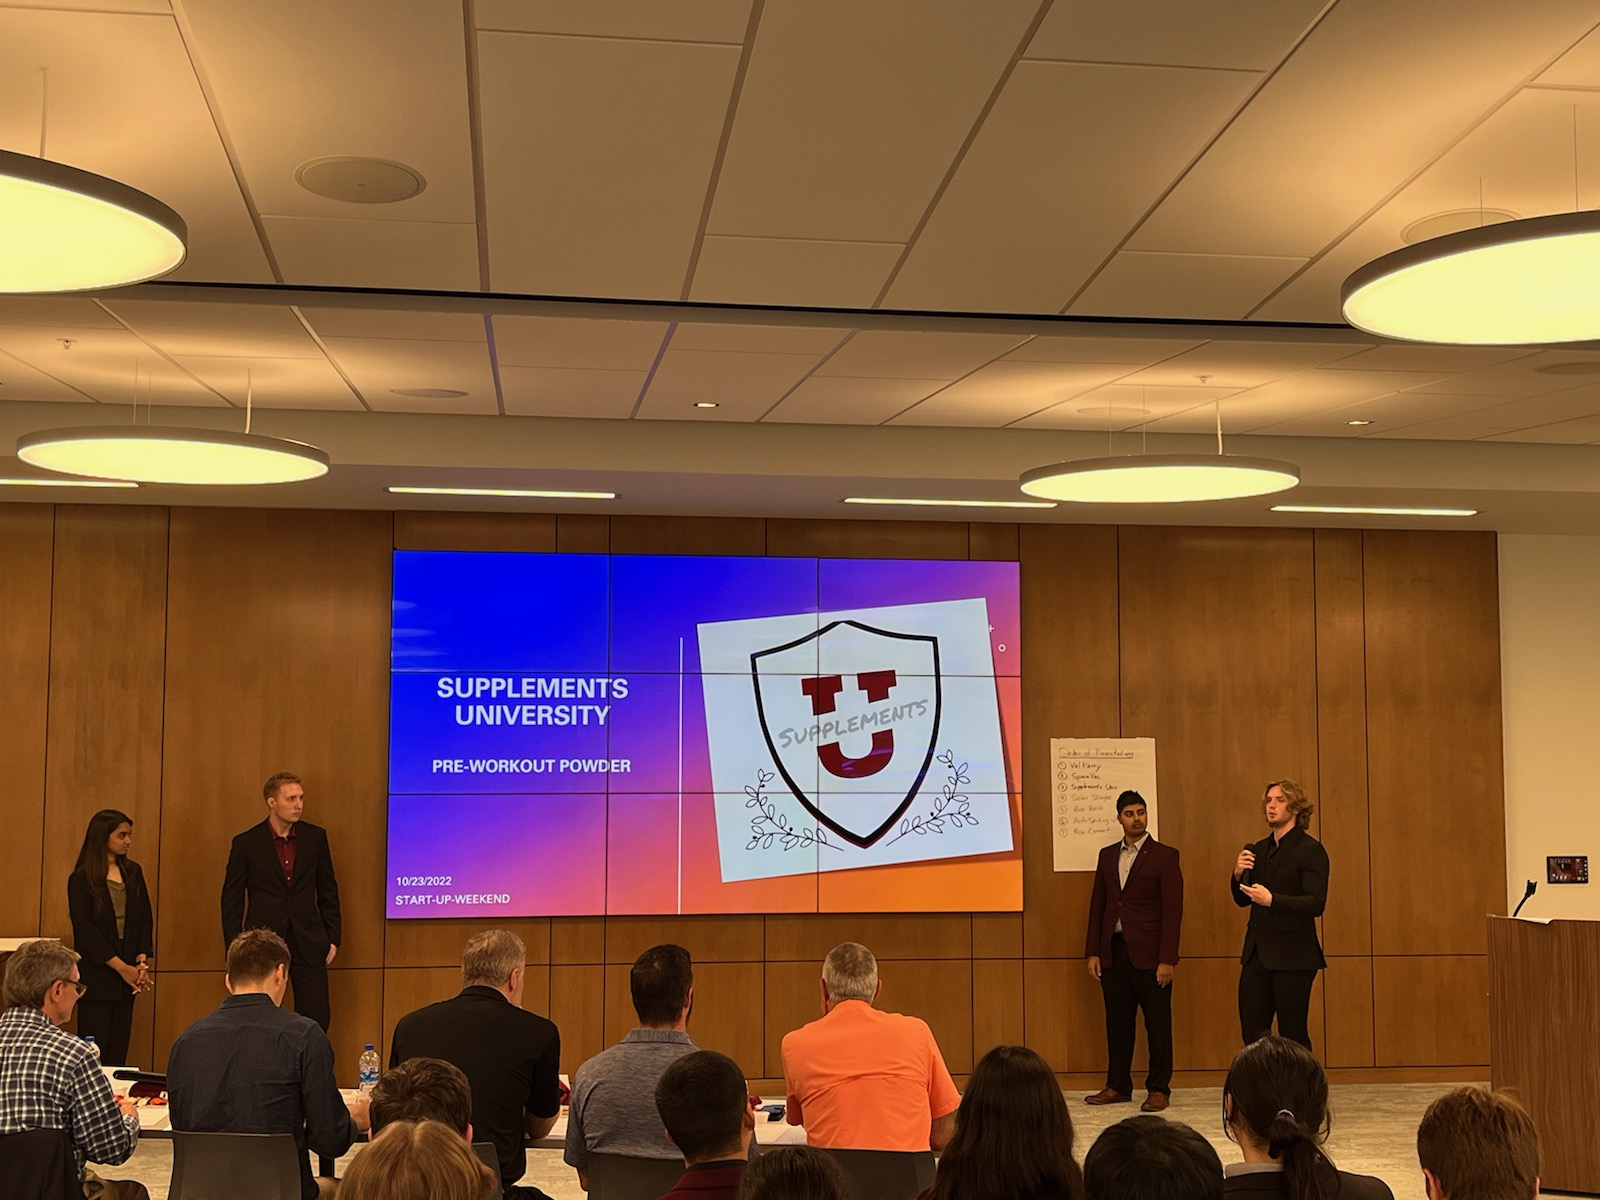
\includegraphics[width=0.5\textwidth]{presentation.jpeg}\end{center}

%-----------------------------------------------------------

\heading{Past Events}{6pt}
\listheading{Activities Fair (8/31)}{0pt}
Before the first day of school, D-Rho hosted a table at the annual Activities Fair, an event designed to attract freshmen interest in Rose's legendary extracurriculars. Prepared with branded pens and stickers, we managed to get 40 responses on our interest survey.
\listheading{Cookout (9/17)}{0pt}
We cooked burgers, met potential new members, and got our name out there. In total, we reached 29 people. 
\listheading{Homecoming (10/8)}{0pt}
D-Rho made an appearance at Rose's famous Tent City, which is a series of tents lining the parking lot just outside the football stadium. We attracted the attention of freshmen, sophomores, parents, and even alumni. 

%-----------------------------------------------------------

\heading{Looking Ahead}{4pt}

\subheading{Recruiting}{2pt}
We have started recruiting new members for next year. We're hoping to have enough new members to lease a second house. We are hosting regular events such as cookouts to attract new members, primarily targeting this year's ESCALATE class.

\subheading{Starting a Speaker Series}{2pt}
We’re looking to host speakers to help further the entrepreneurial education of our members. This series would cover topics such as:
\begin{multicols}{2}
\begin{itemize}
    \item Marketing
    \item How to pitch
    \item How to sell your product
    \item Legal contracts
    \item How to create and manage a team (employees)
    \item Taxes/payroll/ accounting 
    \item How to find investors
    \item When, and if, to sell
    \item Technical entrepreneurship (innovation)
    \item Work-life balance 
    \item Idea generation
    \item Networking 
    \item How to work with a business partner
    \item Corporate entrepreneurship
\end{itemize}
\end{multicols}

\end{minipage} % End the main body - first page mini page